\PassOptionsToPackage{dvipsnames}{xcolor}
\documentclass[border=3mm]{standalone}
\usepackage[dvipsnames]{xcolor}
\usepackage{amsmath}
\usepackage{amssymb}
\usepackage{dsfont}
\usepackage{bm}
\usepackage{tikz}
\usetikzlibrary{arrows}
\usetikzlibrary{calc}

\usepackage{esvect}
\newcommand{\cev}[1]{\reflectbox{\ensuremath{\vv{\reflectbox{\ensuremath{#1}}}}}}


\definecolor{color1}{rgb}{0,0.4470,0.7410}
\definecolor{color2}{rgb}{0.8500,0.3250,0.0980}
\definecolor{color3}{rgb}{0.9290,0.6940,0.1250}
\definecolor{color4}{rgb}{0.4940,0.1840,0.5560}
\definecolor{color5}{rgb}{0.4660,0.6740,0.1880}


\begin{document}



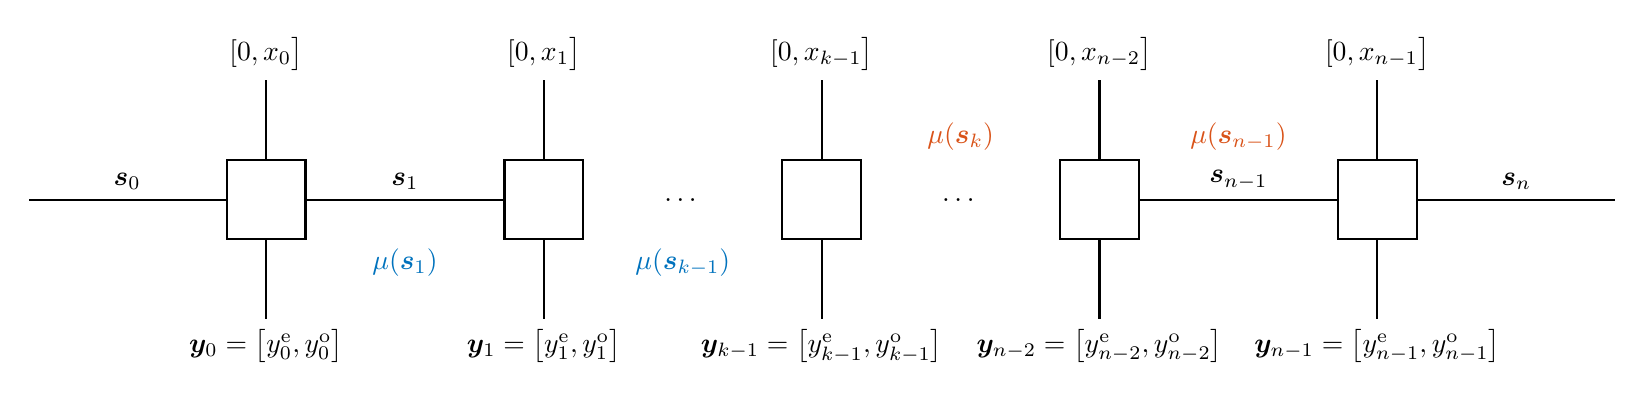
\begin{tikzpicture}[>=stealth,thick]

\node [rectangle, draw, minimum width = 1cm, minimum height = 1cm, anchor=west] (n1) at (0,0) {};
\node [rectangle, draw, minimum width = 1cm, minimum height = 1cm, anchor=west] (n2) at ($(n1.east)+(2.5,0)$) {};
\node [rectangle, draw, minimum width = 1cm, minimum height = 1cm, anchor=west] (n3) at ($(n2.east)+(2.5,0)$) {};
\node [rectangle, draw, minimum width = 1cm, minimum height = 1cm, anchor=west] (n4) at ($(n3.east)+(2.5,0)$) {};
\node [rectangle, draw, minimum width = 1cm, minimum height = 1cm, anchor=west] (n5) at ($(n4.east)+(2.5,0)$) {};


\draw (n1.west) -- node[above] {$\bm s_0$} + (-2.5,0);
\draw (n1.east) --  node[above] {$\bm s_1$} node [color1, yshift=-0.8cm] {$\vv{\mu}(\bm s_1)$}(n2);

\path (n2.east) -- node {$\dotsc$} node [color1,yshift=-0.8cm] {$\vv{\mu}(\bm s_{k-1})$} (n3) ;
\path (n3.east) -- node {$\dotsc$} node [color2,yshift=0.8cm] {$\cev{\mu}(\bm s_{k})$}(n4) ;

\draw (n4.east) -- node[above] {$\bm s_{n-1}$} node [color2,yshift=0.8cm] {$\cev{\mu}(\bm s_{n-1})$}(n5);
\draw (n5.east) -- node[above] {$\bm s_n$}+ (2.5,0);

\draw (n1.south) -- +(0,-1) node[below]{$\bm y_0=\bigl[y_{0}^{\text{e}},y_{0}^{\text{o}}\bigr]$};
\draw (n2.south) -- +(0,-1) node[below]{$\bm y_1=\bigl[y_{1}^{\text{e}},y_{1}^{\text{o}}\bigr]$};
\draw (n3.south) -- +(0,-1) node[below]{$\bm y_{k-1}=\bigl[y_{k-1}^{\text{e}},y_{k-1}^{\text{o}}\bigr]$};
\draw (n4.south) -- +(0,-1) node[below]{$\bm y_{n-2}=\bigl[y_{n-2}^{\text{e}},y_{n-2}^{\text{o}}\bigr]$};
\draw (n5.south) -- +(0,-1) node[below]{$\bm y_{n-1}=\bigl[y_{n-1}^{\text{e}},y_{n-1}^{\text{o}}\bigr]$};

\draw (n1.north) -- +(0,1) node[above]{$[0,x_0\bigr]$};
\draw (n2.north) -- +(0,1) node[above]{$[0,x_1\bigr]$};
\draw (n3.north) -- +(0,1) node[above]{$[0,x_{k-1}\bigr]$};
\draw (n4.north) -- +(0,1) node[above]{$[0,x_{n-2}\bigr]$};
\draw (n5.north) -- +(0,1) node[above]{$[0,x_{n-1}\bigr]$};


\end{tikzpicture}

\end{document}
























